% Created by tikzDevice version 0.12.6 on 2025-04-02 10:50:31
% !TEX encoding = UTF-8 Unicode
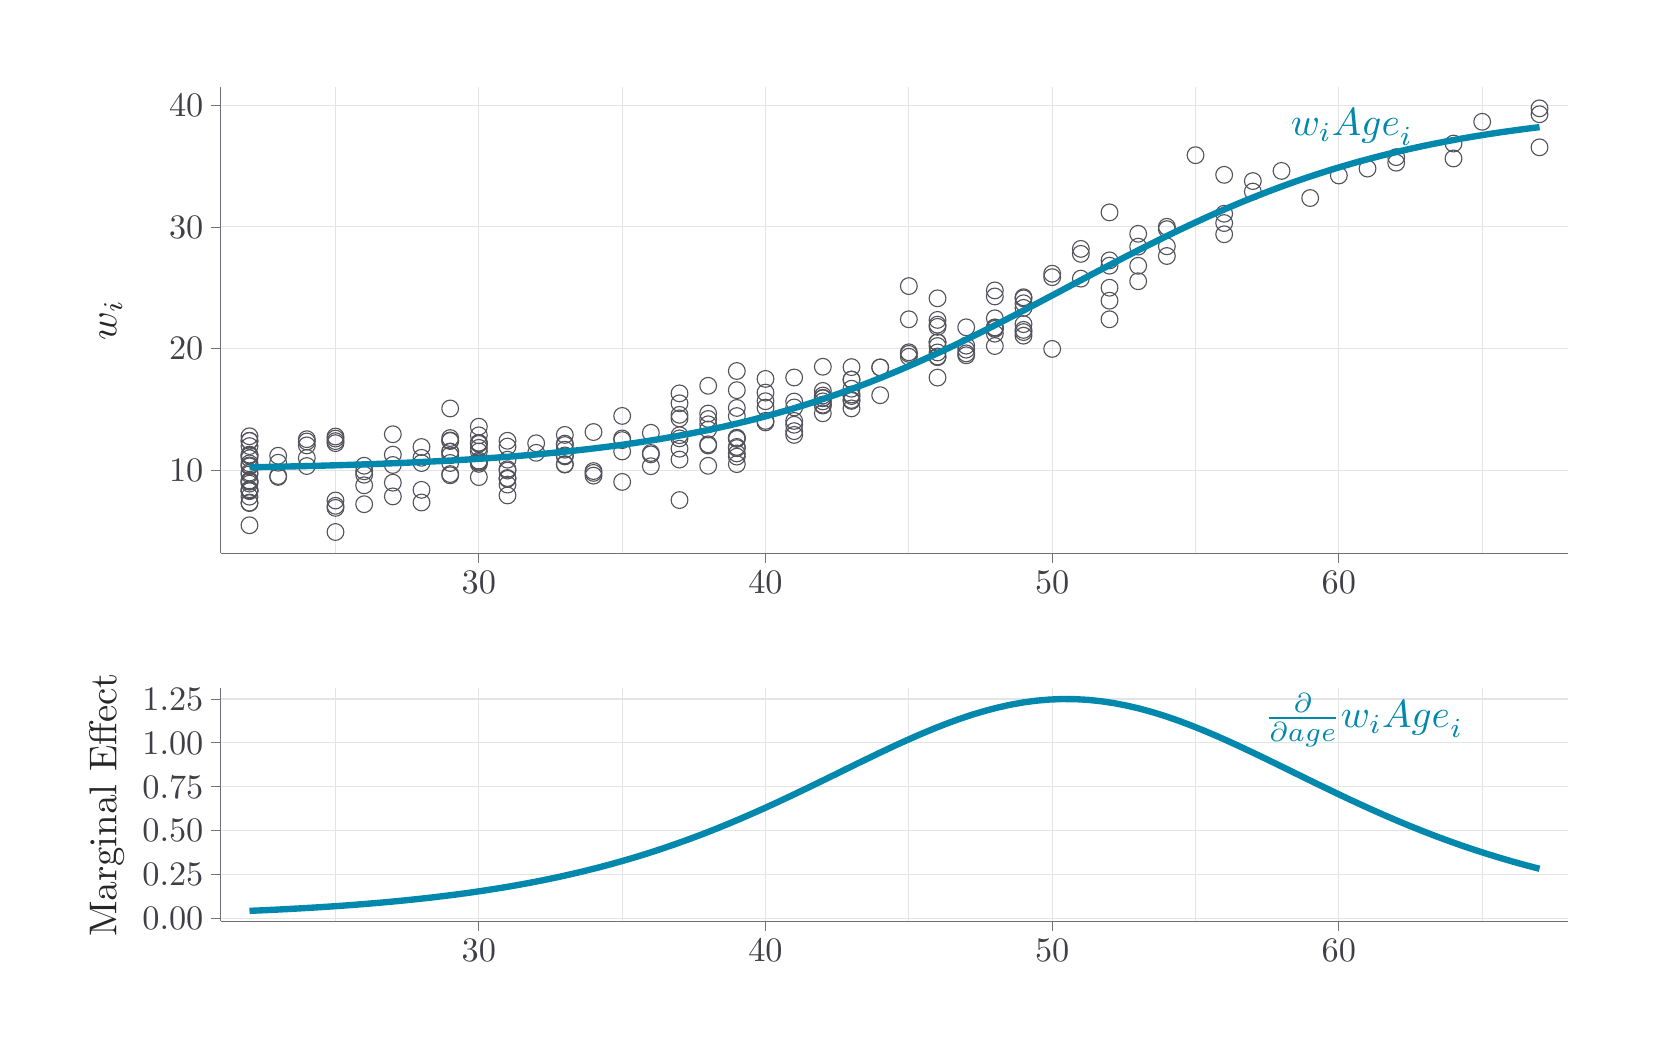
\begin{tikzpicture}[x=1pt,y=1pt]
\definecolor{fillColor}{RGB}{255,255,255}
\path[use as bounding box,fill=fillColor] (0,0) rectangle (578.16,361.35);
\begin{scope}
\path[clip] (  0.00,  0.00) rectangle (578.16,361.35);
\definecolor{drawColor}{RGB}{255,255,255}

\path[draw=drawColor,line width= 0.6pt,line join=round,line cap=round,fill=fillColor] (  0.00,  0.00) rectangle (578.16,361.35);
\end{scope}
\begin{scope}
\path[clip] (  5.50,138.58) rectangle (572.66,355.85);
\definecolor{drawColor}{RGB}{255,255,255}
\definecolor{fillColor}{RGB}{255,255,255}

\path[draw=drawColor,line width= 0.7pt,line join=round,line cap=round,fill=fillColor] (  5.50,138.58) rectangle (572.66,355.85);
\end{scope}
\begin{scope}
\path[clip] (  5.50,  5.50) rectangle (572.66,138.58);
\definecolor{drawColor}{RGB}{255,255,255}
\definecolor{fillColor}{RGB}{255,255,255}

\path[draw=drawColor,line width= 0.7pt,line join=round,line cap=round,fill=fillColor] (  5.50,  5.50) rectangle (572.66,138.58);
\end{scope}
\begin{scope}
\path[clip] ( 69.80,171.46) rectangle (556.66,339.85);
\definecolor{drawColor}{RGB}{255,255,255}
\definecolor{fillColor}{RGB}{255,255,255}

\path[draw=drawColor,line width= 0.7pt,line join=round,line cap=round,fill=fillColor] ( 69.80,171.46) rectangle (556.66,339.85);
\definecolor{drawColor}{RGB}{228,228,231}

\path[draw=drawColor,line width= 0.4pt,line join=round] (111.23,171.46) --
	(111.23,339.85);

\path[draw=drawColor,line width= 0.4pt,line join=round] (214.82,171.46) --
	(214.82,339.85);

\path[draw=drawColor,line width= 0.4pt,line join=round] (318.41,171.46) --
	(318.41,339.85);

\path[draw=drawColor,line width= 0.4pt,line join=round] (422.00,171.46) --
	(422.00,339.85);

\path[draw=drawColor,line width= 0.4pt,line join=round] (525.58,171.46) --
	(525.58,339.85);

\path[draw=drawColor,line width= 0.4pt,line join=round] ( 69.80,201.36) --
	(556.66,201.36);

\path[draw=drawColor,line width= 0.4pt,line join=round] ( 69.80,245.35) --
	(556.66,245.35);

\path[draw=drawColor,line width= 0.4pt,line join=round] ( 69.80,289.34) --
	(556.66,289.34);

\path[draw=drawColor,line width= 0.4pt,line join=round] ( 69.80,333.33) --
	(556.66,333.33);

\path[draw=drawColor,line width= 0.4pt,line join=round] (163.03,171.46) --
	(163.03,339.85);

\path[draw=drawColor,line width= 0.4pt,line join=round] (266.61,171.46) --
	(266.61,339.85);

\path[draw=drawColor,line width= 0.4pt,line join=round] (370.20,171.46) --
	(370.20,339.85);

\path[draw=drawColor,line width= 0.4pt,line join=round] (473.79,171.46) --
	(473.79,339.85);
\definecolor{drawColor}{RGB}{82,82,91}

\path[draw=drawColor,line width= 0.4pt,line join=round,line cap=round] (359.84,252.14) circle (  3.03);

\path[draw=drawColor,line width= 0.4pt,line join=round,line cap=round] (163.03,198.95) circle (  3.03);

\path[draw=drawColor,line width= 0.4pt,line join=round,line cap=round] (194.10,206.77) circle (  3.03);

\path[draw=drawColor,line width= 0.4pt,line join=round,line cap=round] (349.48,246.31) circle (  3.03);

\path[draw=drawColor,line width= 0.4pt,line join=round,line cap=round] (390.92,294.60) circle (  3.03);

\path[draw=drawColor,line width= 0.4pt,line join=round,line cap=round] ( 80.15,203.18) circle (  3.03);

\path[draw=drawColor,line width= 0.4pt,line join=round,line cap=round] ( 80.15,189.56) circle (  3.03);

\path[draw=drawColor,line width= 0.4pt,line join=round,line cap=round] (276.97,219.25) circle (  3.03);

\path[draw=drawColor,line width= 0.4pt,line join=round,line cap=round] (349.48,256.33) circle (  3.03);

\path[draw=drawColor,line width= 0.4pt,line join=round,line cap=round] (370.20,271.19) circle (  3.03);

\path[draw=drawColor,line width= 0.4pt,line join=round,line cap=round] (349.48,252.49) circle (  3.03);

\path[draw=drawColor,line width= 0.4pt,line join=round,line cap=round] (287.33,222.01) circle (  3.03);

\path[draw=drawColor,line width= 0.4pt,line join=round,line cap=round] (256.25,207.50) circle (  3.03);

\path[draw=drawColor,line width= 0.4pt,line join=round,line cap=round] (225.18,207.16) circle (  3.03);

\path[draw=drawColor,line width= 0.4pt,line join=round,line cap=round] (411.64,282.35) circle (  3.03);

\path[draw=drawColor,line width= 0.4pt,line join=round,line cap=round] (194.10,206.42) circle (  3.03);

\path[draw=drawColor,line width= 0.4pt,line join=round,line cap=round] (245.90,218.03) circle (  3.03);

\path[draw=drawColor,line width= 0.4pt,line join=round,line cap=round] (163.03,211.33) circle (  3.03);

\path[draw=drawColor,line width= 0.4pt,line join=round,line cap=round] (245.90,216.15) circle (  3.03);

\path[draw=drawColor,line width= 0.4pt,line join=round,line cap=round] (142.31,194.34) circle (  3.03);

\path[draw=drawColor,line width= 0.4pt,line join=round,line cap=round] (266.61,224.05) circle (  3.03);

\path[draw=drawColor,line width= 0.4pt,line join=round,line cap=round] (328.77,247.64) circle (  3.03);

\path[draw=drawColor,line width= 0.4pt,line join=round,line cap=round] (256.25,213.15) circle (  3.03);

\path[draw=drawColor,line width= 0.4pt,line join=round,line cap=round] (390.92,262.69) circle (  3.03);

\path[draw=drawColor,line width= 0.4pt,line join=round,line cap=round] ( 90.51,206.66) circle (  3.03);

\path[draw=drawColor,line width= 0.4pt,line join=round,line cap=round] (287.33,228.42) circle (  3.03);

\path[draw=drawColor,line width= 0.4pt,line join=round,line cap=round] ( 80.15,205.77) circle (  3.03);

\path[draw=drawColor,line width= 0.4pt,line join=round,line cap=round] (422.00,315.27) circle (  3.03);

\path[draw=drawColor,line width= 0.4pt,line join=round,line cap=round] (308.05,238.58) circle (  3.03);

\path[draw=drawColor,line width= 0.4pt,line join=round,line cap=round] (349.48,264.22) circle (  3.03);

\path[draw=drawColor,line width= 0.4pt,line join=round,line cap=round] (100.87,210.40) circle (  3.03);

\path[draw=drawColor,line width= 0.4pt,line join=round,line cap=round] (349.48,253.04) circle (  3.03);

\path[draw=drawColor,line width= 0.4pt,line join=round,line cap=round] (297.69,228.80) circle (  3.03);

\path[draw=drawColor,line width= 0.4pt,line join=round,line cap=round] (328.77,263.55) circle (  3.03);

\path[draw=drawColor,line width= 0.4pt,line join=round,line cap=round] (131.95,203.33) circle (  3.03);

\path[draw=drawColor,line width= 0.4pt,line join=round,line cap=round] (256.25,209.86) circle (  3.03);

\path[draw=drawColor,line width= 0.4pt,line join=round,line cap=round] (297.69,226.84) circle (  3.03);

\path[draw=drawColor,line width= 0.4pt,line join=round,line cap=round] (390.92,275.35) circle (  3.03);

\path[draw=drawColor,line width= 0.4pt,line join=round,line cap=round] (473.79,307.93) circle (  3.03);

\path[draw=drawColor,line width= 0.4pt,line join=round,line cap=round] (111.23,179.11) circle (  3.03);

\path[draw=drawColor,line width= 0.4pt,line join=round,line cap=round] ( 80.15,199.96) circle (  3.03);

\path[draw=drawColor,line width= 0.4pt,line join=round,line cap=round] (318.41,244.04) circle (  3.03);

\path[draw=drawColor,line width= 0.4pt,line join=round,line cap=round] (235.54,229.20) circle (  3.03);

\path[draw=drawColor,line width= 0.4pt,line join=round,line cap=round] (297.69,226.49) circle (  3.03);

\path[draw=drawColor,line width= 0.4pt,line join=round,line cap=round] (173.38,198.31) circle (  3.03);

\path[draw=drawColor,line width= 0.4pt,line join=round,line cap=round] (235.54,190.65) circle (  3.03);

\path[draw=drawColor,line width= 0.4pt,line join=round,line cap=round] (100.87,205.87) circle (  3.03);

\path[draw=drawColor,line width= 0.4pt,line join=round,line cap=round] (142.31,205.92) circle (  3.03);

\path[draw=drawColor,line width= 0.4pt,line join=round,line cap=round] (380.56,270.66) circle (  3.03);

\path[draw=drawColor,line width= 0.4pt,line join=round,line cap=round] (494.51,314.57) circle (  3.03);

\path[draw=drawColor,line width= 0.4pt,line join=round,line cap=round] (194.10,203.63) circle (  3.03);

\path[draw=drawColor,line width= 0.4pt,line join=round,line cap=round] (515.22,319.47) circle (  3.03);

\path[draw=drawColor,line width= 0.4pt,line join=round,line cap=round] (204.46,200.46) circle (  3.03);

\path[draw=drawColor,line width= 0.4pt,line join=round,line cap=round] (121.59,195.98) circle (  3.03);

\path[draw=drawColor,line width= 0.4pt,line join=round,line cap=round] (297.69,228.25) circle (  3.03);

\path[draw=drawColor,line width= 0.4pt,line join=round,line cap=round] (111.23,211.94) circle (  3.03);

\path[draw=drawColor,line width= 0.4pt,line join=round,line cap=round] (173.38,196.25) circle (  3.03);

\path[draw=drawColor,line width= 0.4pt,line join=round,line cap=round] (173.38,212.07) circle (  3.03);

\path[draw=drawColor,line width= 0.4pt,line join=round,line cap=round] (349.48,250.77) circle (  3.03);

\path[draw=drawColor,line width= 0.4pt,line join=round,line cap=round] (328.77,254.03) circle (  3.03);

\path[draw=drawColor,line width= 0.4pt,line join=round,line cap=round] (339.13,245.01) circle (  3.03);

\path[draw=drawColor,line width= 0.4pt,line join=round,line cap=round] (111.23,190.49) circle (  3.03);

\path[draw=drawColor,line width= 0.4pt,line join=round,line cap=round] (152.67,212.00) circle (  3.03);

\path[draw=drawColor,line width= 0.4pt,line join=round,line cap=round] ( 80.15,189.73) circle (  3.03);

\path[draw=drawColor,line width= 0.4pt,line join=round,line cap=round] (266.61,226.37) circle (  3.03);

\path[draw=drawColor,line width= 0.4pt,line join=round,line cap=round] (276.97,224.11) circle (  3.03);

\path[draw=drawColor,line width= 0.4pt,line join=round,line cap=round] (276.97,234.94) circle (  3.03);

\path[draw=drawColor,line width= 0.4pt,line join=round,line cap=round] (494.51,312.54) circle (  3.03);

\path[draw=drawColor,line width= 0.4pt,line join=round,line cap=round] (266.61,229.48) circle (  3.03);

\path[draw=drawColor,line width= 0.4pt,line join=round,line cap=round] (111.23,213.61) circle (  3.03);

\path[draw=drawColor,line width= 0.4pt,line join=round,line cap=round] (546.30,330.06) circle (  3.03);

\path[draw=drawColor,line width= 0.4pt,line join=round,line cap=round] (235.54,214.09) circle (  3.03);

\path[draw=drawColor,line width= 0.4pt,line join=round,line cap=round] (131.95,214.43) circle (  3.03);

\path[draw=drawColor,line width= 0.4pt,line join=round,line cap=round] (287.33,238.82) circle (  3.03);

\path[draw=drawColor,line width= 0.4pt,line join=round,line cap=round] (152.67,208.06) circle (  3.03);

\path[draw=drawColor,line width= 0.4pt,line join=round,line cap=round] (245.90,221.91) circle (  3.03);

\path[draw=drawColor,line width= 0.4pt,line join=round,line cap=round] ( 80.15,203.90) circle (  3.03);

\path[draw=drawColor,line width= 0.4pt,line join=round,line cap=round] ( 80.15,196.59) circle (  3.03);

\path[draw=drawColor,line width= 0.4pt,line join=round,line cap=round] (359.84,263.53) circle (  3.03);

\path[draw=drawColor,line width= 0.4pt,line join=round,line cap=round] (546.30,318.11) circle (  3.03);

\path[draw=drawColor,line width= 0.4pt,line join=round,line cap=round] (204.46,199.48) circle (  3.03);

\path[draw=drawColor,line width= 0.4pt,line join=round,line cap=round] ( 80.15,197.30) circle (  3.03);

\path[draw=drawColor,line width= 0.4pt,line join=round,line cap=round] (204.46,201.13) circle (  3.03);

\path[draw=drawColor,line width= 0.4pt,line join=round,line cap=round] (214.82,208.21) circle (  3.03);

\path[draw=drawColor,line width= 0.4pt,line join=round,line cap=round] (349.48,266.41) circle (  3.03);

\path[draw=drawColor,line width= 0.4pt,line join=round,line cap=round] (401.28,275.30) circle (  3.03);

\path[draw=drawColor,line width= 0.4pt,line join=round,line cap=round] (328.77,253.24) circle (  3.03);

\path[draw=drawColor,line width= 0.4pt,line join=round,line cap=round] ( 80.15,212.01) circle (  3.03);

\path[draw=drawColor,line width= 0.4pt,line join=round,line cap=round] (173.38,198.61) circle (  3.03);

\path[draw=drawColor,line width= 0.4pt,line join=round,line cap=round] (214.82,221.05) circle (  3.03);

\path[draw=drawColor,line width= 0.4pt,line join=round,line cap=round] (339.13,253.07) circle (  3.03);

\path[draw=drawColor,line width= 0.4pt,line join=round,line cap=round] (131.95,196.93) circle (  3.03);

\path[draw=drawColor,line width= 0.4pt,line join=round,line cap=round] (142.31,189.77) circle (  3.03);

\path[draw=drawColor,line width= 0.4pt,line join=round,line cap=round] (256.25,213.12) circle (  3.03);

\path[draw=drawColor,line width= 0.4pt,line join=round,line cap=round] (204.46,215.23) circle (  3.03);

\path[draw=drawColor,line width= 0.4pt,line join=round,line cap=round] (276.97,214.19) circle (  3.03);

\path[draw=drawColor,line width= 0.4pt,line join=round,line cap=round] (173.38,201.30) circle (  3.03);

\path[draw=drawColor,line width= 0.4pt,line join=round,line cap=round] (432.35,294.11) circle (  3.03);

\path[draw=drawColor,line width= 0.4pt,line join=round,line cap=round] (287.33,224.80) circle (  3.03);

\path[draw=drawColor,line width= 0.4pt,line join=round,line cap=round] (100.87,202.95) circle (  3.03);

\path[draw=drawColor,line width= 0.4pt,line join=round,line cap=round] (411.64,289.39) circle (  3.03);

\path[draw=drawColor,line width= 0.4pt,line join=round,line cap=round] (235.54,220.16) circle (  3.03);

\path[draw=drawColor,line width= 0.4pt,line join=round,line cap=round] (100.87,212.64) circle (  3.03);

\path[draw=drawColor,line width= 0.4pt,line join=round,line cap=round] ( 90.51,204.14) circle (  3.03);

\path[draw=drawColor,line width= 0.4pt,line join=round,line cap=round] (401.28,282.23) circle (  3.03);

\path[draw=drawColor,line width= 0.4pt,line join=round,line cap=round] (163.03,210.93) circle (  3.03);

\path[draw=drawColor,line width= 0.4pt,line join=round,line cap=round] (359.84,254.23) circle (  3.03);

\path[draw=drawColor,line width= 0.4pt,line join=round,line cap=round] (297.69,230.88) circle (  3.03);

\path[draw=drawColor,line width= 0.4pt,line join=round,line cap=round] (266.61,219.26) circle (  3.03);

\path[draw=drawColor,line width= 0.4pt,line join=round,line cap=round] (453.07,309.59) circle (  3.03);

\path[draw=drawColor,line width= 0.4pt,line join=round,line cap=round] (380.56,279.61) circle (  3.03);

\path[draw=drawColor,line width= 0.4pt,line join=round,line cap=round] ( 80.15,207.07) circle (  3.03);

\path[draw=drawColor,line width= 0.4pt,line join=round,line cap=round] (256.25,221.00) circle (  3.03);

\path[draw=drawColor,line width= 0.4pt,line join=round,line cap=round] ( 80.15,194.53) circle (  3.03);

\path[draw=drawColor,line width= 0.4pt,line join=round,line cap=round] (328.77,255.75) circle (  3.03);

\path[draw=drawColor,line width= 0.4pt,line join=round,line cap=round] (256.25,206.35) circle (  3.03);

\path[draw=drawColor,line width= 0.4pt,line join=round,line cap=round] (121.59,199.80) circle (  3.03);

\path[draw=drawColor,line width= 0.4pt,line join=round,line cap=round] (163.03,204.87) circle (  3.03);

\path[draw=drawColor,line width= 0.4pt,line join=round,line cap=round] (390.92,277.25) circle (  3.03);

\path[draw=drawColor,line width= 0.4pt,line join=round,line cap=round] ( 90.51,199.36) circle (  3.03);

\path[draw=drawColor,line width= 0.4pt,line join=round,line cap=round] (297.69,234.16) circle (  3.03);

\path[draw=drawColor,line width= 0.4pt,line join=round,line cap=round] (339.13,242.97) circle (  3.03);

\path[draw=drawColor,line width= 0.4pt,line join=round,line cap=round] (380.56,281.41) circle (  3.03);

\path[draw=drawColor,line width= 0.4pt,line join=round,line cap=round] (235.54,225.62) circle (  3.03);

\path[draw=drawColor,line width= 0.4pt,line join=round,line cap=round] (214.82,212.31) circle (  3.03);

\path[draw=drawColor,line width= 0.4pt,line join=round,line cap=round] (266.61,234.43) circle (  3.03);

\path[draw=drawColor,line width= 0.4pt,line join=round,line cap=round] (152.67,223.75) circle (  3.03);

\path[draw=drawColor,line width= 0.4pt,line join=round,line cap=round] (390.92,267.37) circle (  3.03);

\path[draw=drawColor,line width= 0.4pt,line join=round,line cap=round] (442.71,305.92) circle (  3.03);

\path[draw=drawColor,line width= 0.4pt,line join=round,line cap=round] (463.43,299.78) circle (  3.03);

\path[draw=drawColor,line width= 0.4pt,line join=round,line cap=round] (111.23,212.87) circle (  3.03);

\path[draw=drawColor,line width= 0.4pt,line join=round,line cap=round] (370.20,272.45) circle (  3.03);

\path[draw=drawColor,line width= 0.4pt,line join=round,line cap=round] (328.77,246.31) circle (  3.03);

\path[draw=drawColor,line width= 0.4pt,line join=round,line cap=round] (349.48,252.87) circle (  3.03);

\path[draw=drawColor,line width= 0.4pt,line join=round,line cap=round] ( 80.15,181.54) circle (  3.03);

\path[draw=drawColor,line width= 0.4pt,line join=round,line cap=round] ( 80.15,193.89) circle (  3.03);

\path[draw=drawColor,line width= 0.4pt,line join=round,line cap=round] (266.61,218.71) circle (  3.03);

\path[draw=drawColor,line width= 0.4pt,line join=round,line cap=round] (308.05,238.56) circle (  3.03);

\path[draw=drawColor,line width= 0.4pt,line join=round,line cap=round] (411.64,288.54) circle (  3.03);

\path[draw=drawColor,line width= 0.4pt,line join=round,line cap=round] (297.69,234.21) circle (  3.03);

\path[draw=drawColor,line width= 0.4pt,line join=round,line cap=round] (287.33,227.58) circle (  3.03);

\path[draw=drawColor,line width= 0.4pt,line join=round,line cap=round] (163.03,214.05) circle (  3.03);

\path[draw=drawColor,line width= 0.4pt,line join=round,line cap=round] (245.90,210.80) circle (  3.03);

\path[draw=drawColor,line width= 0.4pt,line join=round,line cap=round] (111.23,188.57) circle (  3.03);

\path[draw=drawColor,line width= 0.4pt,line join=round,line cap=round] (359.84,251.35) circle (  3.03);

\path[draw=drawColor,line width= 0.4pt,line join=round,line cap=round] (484.15,310.43) circle (  3.03);

\path[draw=drawColor,line width= 0.4pt,line join=round,line cap=round] (256.25,230.36) circle (  3.03);

\path[draw=drawColor,line width= 0.4pt,line join=round,line cap=round] (152.67,204.05) circle (  3.03);

\path[draw=drawColor,line width= 0.4pt,line join=round,line cap=round] (287.33,226.31) circle (  3.03);

\path[draw=drawColor,line width= 0.4pt,line join=round,line cap=round] ( 80.15,212.08) circle (  3.03);

\path[draw=drawColor,line width= 0.4pt,line join=round,line cap=round] (318.41,267.97) circle (  3.03);

\path[draw=drawColor,line width= 0.4pt,line join=round,line cap=round] (297.69,238.68) circle (  3.03);

\path[draw=drawColor,line width= 0.4pt,line join=round,line cap=round] (339.13,246.44) circle (  3.03);

\path[draw=drawColor,line width= 0.4pt,line join=round,line cap=round] (370.20,245.27) circle (  3.03);

\path[draw=drawColor,line width= 0.4pt,line join=round,line cap=round] (276.97,215.56) circle (  3.03);

\path[draw=drawColor,line width= 0.4pt,line join=round,line cap=round] (256.25,237.28) circle (  3.03);

\path[draw=drawColor,line width= 0.4pt,line join=round,line cap=round] (214.82,197.21) circle (  3.03);

\path[draw=drawColor,line width= 0.4pt,line join=round,line cap=round] (111.23,187.82) circle (  3.03);

\path[draw=drawColor,line width= 0.4pt,line join=round,line cap=round] (152.67,206.82) circle (  3.03);

\path[draw=drawColor,line width= 0.4pt,line join=round,line cap=round] (183.74,211.17) circle (  3.03);

\path[draw=drawColor,line width= 0.4pt,line join=round,line cap=round] (328.77,234.90) circle (  3.03);

\path[draw=drawColor,line width= 0.4pt,line join=round,line cap=round] (359.84,250.05) circle (  3.03);

\path[draw=drawColor,line width= 0.4pt,line join=round,line cap=round] ( 80.15,202.81) circle (  3.03);

\path[draw=drawColor,line width= 0.4pt,line join=round,line cap=round] ( 80.15,193.98) circle (  3.03);

\path[draw=drawColor,line width= 0.4pt,line join=round,line cap=round] (297.69,223.77) circle (  3.03);

\path[draw=drawColor,line width= 0.4pt,line join=round,line cap=round] (432.35,286.69) circle (  3.03);

\path[draw=drawColor,line width= 0.4pt,line join=round,line cap=round] (276.97,217.86) circle (  3.03);

\path[draw=drawColor,line width= 0.4pt,line join=round,line cap=round] (121.59,203.05) circle (  3.03);

\path[draw=drawColor,line width= 0.4pt,line join=round,line cap=round] (163.03,204.37) circle (  3.03);

\path[draw=drawColor,line width= 0.4pt,line join=round,line cap=round] (525.58,327.34) circle (  3.03);

\path[draw=drawColor,line width= 0.4pt,line join=round,line cap=round] (142.31,204.03) circle (  3.03);

\path[draw=drawColor,line width= 0.4pt,line join=round,line cap=round] (401.28,269.72) circle (  3.03);

\path[draw=drawColor,line width= 0.4pt,line join=round,line cap=round] ( 80.15,206.70) circle (  3.03);

\path[draw=drawColor,line width= 0.4pt,line join=round,line cap=round] (131.95,207.05) circle (  3.03);

\path[draw=drawColor,line width= 0.4pt,line join=round,line cap=round] (287.33,227.43) circle (  3.03);

\path[draw=drawColor,line width= 0.4pt,line join=round,line cap=round] (235.54,209.21) circle (  3.03);

\path[draw=drawColor,line width= 0.4pt,line join=round,line cap=round] (173.38,201.80) circle (  3.03);

\path[draw=drawColor,line width= 0.4pt,line join=round,line cap=round] (401.28,286.86) circle (  3.03);

\path[draw=drawColor,line width= 0.4pt,line join=round,line cap=round] (287.33,230.09) circle (  3.03);

\path[draw=drawColor,line width= 0.4pt,line join=round,line cap=round] (163.03,211.26) circle (  3.03);

\path[draw=drawColor,line width= 0.4pt,line join=round,line cap=round] (152.67,213.06) circle (  3.03);

\path[draw=drawColor,line width= 0.4pt,line join=round,line cap=round] (359.84,263.94) circle (  3.03);

\path[draw=drawColor,line width= 0.4pt,line join=round,line cap=round] (111.23,211.22) circle (  3.03);

\path[draw=drawColor,line width= 0.4pt,line join=round,line cap=round] (183.74,207.72) circle (  3.03);

\path[draw=drawColor,line width= 0.4pt,line join=round,line cap=round] (339.13,243.65) circle (  3.03);

\path[draw=drawColor,line width= 0.4pt,line join=round,line cap=round] (442.71,302.12) circle (  3.03);

\path[draw=drawColor,line width= 0.4pt,line join=round,line cap=round] (194.10,203.47) circle (  3.03);

\path[draw=drawColor,line width= 0.4pt,line join=round,line cap=round] (152.67,200.05) circle (  3.03);

\path[draw=drawColor,line width= 0.4pt,line join=round,line cap=round] (225.18,214.95) circle (  3.03);

\path[draw=drawColor,line width= 0.4pt,line join=round,line cap=round] (256.25,209.43) circle (  3.03);

\path[draw=drawColor,line width= 0.4pt,line join=round,line cap=round] (245.90,210.36) circle (  3.03);

\path[draw=drawColor,line width= 0.4pt,line join=round,line cap=round] (256.25,223.93) circle (  3.03);

\path[draw=drawColor,line width= 0.4pt,line join=round,line cap=round] (100.87,211.81) circle (  3.03);

\path[draw=drawColor,line width= 0.4pt,line join=round,line cap=round] ( 90.51,199.00) circle (  3.03);

\path[draw=drawColor,line width= 0.4pt,line join=round,line cap=round] (256.25,203.64) circle (  3.03);

\path[draw=drawColor,line width= 0.4pt,line join=round,line cap=round] (328.77,247.65) circle (  3.03);

\path[draw=drawColor,line width= 0.4pt,line join=round,line cap=round] (163.03,209.52) circle (  3.03);

\path[draw=drawColor,line width= 0.4pt,line join=round,line cap=round] (173.38,209.98) circle (  3.03);

\path[draw=drawColor,line width= 0.4pt,line join=round,line cap=round] (276.97,226.24) circle (  3.03);

\path[draw=drawColor,line width= 0.4pt,line join=round,line cap=round] (318.41,255.97) circle (  3.03);

\path[draw=drawColor,line width= 0.4pt,line join=round,line cap=round] (131.95,191.97) circle (  3.03);

\path[draw=drawColor,line width= 0.4pt,line join=round,line cap=round] (225.18,207.66) circle (  3.03);

\path[draw=drawColor,line width= 0.4pt,line join=round,line cap=round] (318.41,243.47) circle (  3.03);

\path[draw=drawColor,line width= 0.4pt,line join=round,line cap=round] (256.25,212.74) circle (  3.03);

\path[draw=drawColor,line width= 0.4pt,line join=round,line cap=round] (359.84,260.09) circle (  3.03);

\path[draw=drawColor,line width= 0.4pt,line join=round,line cap=round] (163.03,217.16) circle (  3.03);

\path[draw=drawColor,line width= 0.4pt,line join=round,line cap=round] (152.67,199.60) circle (  3.03);

\path[draw=drawColor,line width= 0.4pt,line join=round,line cap=round] (142.31,209.82) circle (  3.03);

\path[draw=drawColor,line width= 0.4pt,line join=round,line cap=round] (152.67,208.19) circle (  3.03);

\path[draw=drawColor,line width= 0.4pt,line join=round,line cap=round] (225.18,202.88) circle (  3.03);

\path[draw=drawColor,line width= 0.4pt,line join=round,line cap=round] (411.64,278.84) circle (  3.03);

\path[draw=drawColor,line width= 0.4pt,line join=round,line cap=round] ( 80.15,197.71) circle (  3.03);

\path[draw=drawColor,line width= 0.4pt,line join=round,line cap=round] ( 80.15,213.70) circle (  3.03);

\path[draw=drawColor,line width= 0.4pt,line join=round,line cap=round] (121.59,189.15) circle (  3.03);

\path[draw=drawColor,line width= 0.4pt,line join=round,line cap=round] (359.84,261.76) circle (  3.03);

\path[draw=drawColor,line width= 0.4pt,line join=round,line cap=round] (245.90,203.03) circle (  3.03);

\path[draw=drawColor,line width= 0.4pt,line join=round,line cap=round] (328.77,243.99) circle (  3.03);

\path[draw=drawColor,line width= 0.4pt,line join=round,line cap=round] (546.30,332.20) circle (  3.03);

\path[draw=drawColor,line width= 0.4pt,line join=round,line cap=round] (194.10,211.04) circle (  3.03);

\path[draw=drawColor,line width= 0.4pt,line join=round,line cap=round] (173.38,205.24) circle (  3.03);

\path[draw=drawColor,line width= 0.4pt,line join=round,line cap=round] (245.90,219.94) circle (  3.03);

\path[draw=drawColor,line width= 0.4pt,line join=round,line cap=round] (235.54,221.45) circle (  3.03);

\path[draw=drawColor,line width= 0.4pt,line join=round,line cap=round] (194.10,214.19) circle (  3.03);

\path[draw=drawColor,line width= 0.4pt,line join=round,line cap=round] (308.05,228.54) circle (  3.03);

\path[draw=drawColor,line width= 0.4pt,line join=round,line cap=round] ( 80.15,200.59) circle (  3.03);

\path[draw=drawColor,line width= 0.4pt,line join=round,line cap=round] (318.41,242.43) circle (  3.03);

\path[draw=drawColor,line width= 0.4pt,line join=round,line cap=round] (163.03,208.22) circle (  3.03);

\path[draw=drawColor,line width= 0.4pt,line join=round,line cap=round] ( 80.15,197.41) circle (  3.03);

\path[draw=drawColor,line width= 0.4pt,line join=round,line cap=round] (121.59,201.05) circle (  3.03);

\path[draw=drawColor,line width= 0.4pt,line join=round,line cap=round] ( 80.15,206.72) circle (  3.03);

\path[draw=drawColor,line width= 0.4pt,line join=round,line cap=round] (245.90,231.94) circle (  3.03);

\path[draw=drawColor,line width= 0.4pt,line join=round,line cap=round] (235.54,212.94) circle (  3.03);

\path[draw=drawColor,line width= 0.4pt,line join=round,line cap=round] ( 80.15,194.10) circle (  3.03);

\path[draw=drawColor,line width= 0.4pt,line join=round,line cap=round] (328.77,242.28) circle (  3.03);

\path[draw=drawColor,line width= 0.4pt,line join=round,line cap=round] (432.35,290.75) circle (  3.03);

\path[draw=drawColor,line width= 0.4pt,line join=round,line cap=round] (515.22,314.08) circle (  3.03);

\path[draw=drawColor,line width= 0.4pt,line join=round,line cap=round] (390.92,255.97) circle (  3.03);

\path[draw=drawColor,line width= 0.4pt,line join=round,line cap=round] (432.35,308.17) circle (  3.03);

\path[draw=drawColor,line width= 0.4pt,line join=round,line cap=round] (194.10,210.53) circle (  3.03);

\path[draw=drawColor,line width= 0.4pt,line join=round,line cap=round] (163.03,203.74) circle (  3.03);

\path[draw=drawColor,line width= 0.4pt,line join=round,line cap=round] ( 80.15,210.15) circle (  3.03);

\path[draw=drawColor,line width= 0.4pt,line join=round,line cap=round] (287.33,225.12) circle (  3.03);

\path[draw=drawColor,line width= 0.4pt,line join=round,line cap=round] (235.54,205.28) circle (  3.03);

\path[draw=drawColor,line width= 0.4pt,line join=round,line cap=round] (163.03,204.32) circle (  3.03);

\path[draw=drawColor,line width= 0.4pt,line join=round,line cap=round] (214.82,212.92) circle (  3.03);

\path[draw=drawColor,line width= 0.4pt,line join=round,line cap=round] (173.38,192.32) circle (  3.03);

\path[draw=drawColor,line width= 0.4pt,line join=round,line cap=round] (328.77,242.52) circle (  3.03);

\path[draw=drawColor,line width= 0.4pt,line join=round,line cap=round] (152.67,212.18) circle (  3.03);

\path[draw=drawColor,line width= 0.4pt,line join=round,line cap=round] (194.10,208.85) circle (  3.03);

\path[draw=drawColor,line width= 0.4pt,line join=round,line cap=round] ( 80.15,191.87) circle (  3.03);
\definecolor{drawColor}{RGB}{1,136,172}

\path[draw=drawColor,line width= 2.3pt,line join=round] ( 80.15,202.49) --
	( 84.82,202.58) --
	( 89.48,202.67) --
	( 94.14,202.78) --
	( 98.80,202.88) --
	(103.46,203.00) --
	(108.12,203.13) --
	(112.79,203.26) --
	(117.45,203.41) --
	(122.11,203.57) --
	(126.77,203.73) --
	(131.43,203.92) --
	(136.09,204.11) --
	(140.75,204.32) --
	(145.42,204.55) --
	(150.08,204.79) --
	(154.74,205.05) --
	(159.40,205.32) --
	(164.06,205.62) --
	(168.72,205.94) --
	(173.38,206.29) --
	(178.05,206.66) --
	(182.71,207.05) --
	(187.37,207.47) --
	(192.03,207.93) --
	(196.69,208.41) --
	(201.35,208.93) --
	(206.01,209.48) --
	(210.68,210.07) --
	(215.34,210.70) --
	(220.00,211.37) --
	(224.66,212.09) --
	(229.32,212.85) --
	(233.98,213.66) --
	(238.64,214.53) --
	(243.31,215.44) --
	(247.97,216.41) --
	(252.63,217.44) --
	(257.29,218.53) --
	(261.95,219.68) --
	(266.61,220.90) --
	(271.27,222.18) --
	(275.94,223.53) --
	(280.60,224.95) --
	(285.26,226.44) --
	(289.92,228.00) --
	(294.58,229.63) --
	(299.24,231.33) --
	(303.91,233.10) --
	(308.57,234.94) --
	(313.23,236.85) --
	(317.89,238.83) --
	(322.55,240.88) --
	(327.21,242.99) --
	(331.87,245.15) --
	(336.54,247.37) --
	(341.20,249.65) --
	(345.86,251.96) --
	(350.52,254.32) --
	(355.18,256.72) --
	(359.84,259.14) --
	(364.50,261.59) --
	(369.17,264.05) --
	(373.83,266.52) --
	(378.49,269.00) --
	(383.15,271.47) --
	(387.81,273.92) --
	(392.47,276.36) --
	(397.13,278.78) --
	(401.80,281.16) --
	(406.46,283.51) --
	(411.12,285.81) --
	(415.78,288.07) --
	(420.44,290.27) --
	(425.10,292.42) --
	(429.76,294.51) --
	(434.43,296.53) --
	(439.09,298.49) --
	(443.75,300.38) --
	(448.41,302.19) --
	(453.07,303.94) --
	(457.73,305.62) --
	(462.39,307.23) --
	(467.06,308.76) --
	(471.72,310.23) --
	(476.38,311.62) --
	(481.04,312.95) --
	(485.70,314.21) --
	(490.36,315.40) --
	(495.03,316.53) --
	(499.69,317.60) --
	(504.35,318.61) --
	(509.01,319.56) --
	(513.67,320.46) --
	(518.33,321.31) --
	(522.99,322.10) --
	(527.66,322.85) --
	(532.32,323.55) --
	(536.98,324.21) --
	(541.64,324.83) --
	(546.30,325.40);

\path[] (425.18,317.97) --
	(502.30,317.97) --
	(502.19,317.97) --
	(502.61,317.99) --
	(503.01,318.07) --
	(503.40,318.22) --
	(503.76,318.43) --
	(504.08,318.69) --
	(504.35,319.00) --
	(504.57,319.35) --
	(504.73,319.73) --
	(504.83,320.13) --
	(504.87,320.54) --
	(504.87,320.54) --
	(504.87,333.30) --
	(504.87,333.30) --
	(504.83,333.72) --
	(504.73,334.12) --
	(504.57,334.50) --
	(504.35,334.85) --
	(504.08,335.16) --
	(503.76,335.42) --
	(503.40,335.63) --
	(503.01,335.77) --
	(502.61,335.86) --
	(502.30,335.87) --
	(425.18,335.87) --
	(425.49,335.86) --
	(425.08,335.87) --
	(424.66,335.82) --
	(424.27,335.71) --
	(423.89,335.53) --
	(423.55,335.29) --
	(423.26,335.01) --
	(423.01,334.68) --
	(422.81,334.31) --
	(422.68,333.92) --
	(422.62,333.51) --
	(422.61,333.30) --
	(422.61,320.54) --
	(422.62,320.75) --
	(422.62,320.34) --
	(422.68,319.93) --
	(422.81,319.53) --
	(423.01,319.17) --
	(423.26,318.84) --
	(423.55,318.55) --
	(423.89,318.32) --
	(424.27,318.14) --
	(424.66,318.02) --
	(425.08,317.97) --
	cycle;
\end{scope}
\begin{scope}
\path[clip] ( 69.80,171.46) rectangle (556.66,339.85);
\definecolor{drawColor}{RGB}{1,136,172}

\node[text=drawColor,anchor=base east,inner sep=0pt, outer sep=0pt, scale=  1.42] at (500.58,322.26) {$\expec{w_i}{\text{Age}_i}$};
\end{scope}
\begin{scope}
\path[clip] (  0.00,  0.00) rectangle (578.16,361.35);
\definecolor{drawColor}{RGB}{113,113,122}

\path[draw=drawColor,line width= 0.3pt,line join=round] ( 69.80,171.46) --
	( 69.80,339.85);
\end{scope}
\begin{scope}
\path[clip] (  0.00,  0.00) rectangle (578.16,361.35);
\definecolor{drawColor}{RGB}{63,63,70}

\node[text=drawColor,anchor=base east,inner sep=0pt, outer sep=0pt, scale=  1.24] at ( 63.50,197.28) {10};

\node[text=drawColor,anchor=base east,inner sep=0pt, outer sep=0pt, scale=  1.24] at ( 63.50,241.27) {20};

\node[text=drawColor,anchor=base east,inner sep=0pt, outer sep=0pt, scale=  1.24] at ( 63.50,285.26) {30};

\node[text=drawColor,anchor=base east,inner sep=0pt, outer sep=0pt, scale=  1.24] at ( 63.50,329.25) {40};
\end{scope}
\begin{scope}
\path[clip] (  0.00,  0.00) rectangle (578.16,361.35);
\definecolor{drawColor}{RGB}{113,113,122}

\path[draw=drawColor,line width= 0.3pt,line join=round] ( 66.30,201.36) --
	( 69.80,201.36);

\path[draw=drawColor,line width= 0.3pt,line join=round] ( 66.30,245.35) --
	( 69.80,245.35);

\path[draw=drawColor,line width= 0.3pt,line join=round] ( 66.30,289.34) --
	( 69.80,289.34);

\path[draw=drawColor,line width= 0.3pt,line join=round] ( 66.30,333.33) --
	( 69.80,333.33);
\end{scope}
\begin{scope}
\path[clip] (  0.00,  0.00) rectangle (578.16,361.35);
\definecolor{drawColor}{RGB}{113,113,122}

\path[draw=drawColor,line width= 0.3pt,line join=round] ( 69.80,171.46) --
	(556.66,171.46);
\end{scope}
\begin{scope}
\path[clip] (  0.00,  0.00) rectangle (578.16,361.35);
\definecolor{drawColor}{RGB}{113,113,122}

\path[draw=drawColor,line width= 0.3pt,line join=round] (163.03,167.96) --
	(163.03,171.46);

\path[draw=drawColor,line width= 0.3pt,line join=round] (266.61,167.96) --
	(266.61,171.46);

\path[draw=drawColor,line width= 0.3pt,line join=round] (370.20,167.96) --
	(370.20,171.46);

\path[draw=drawColor,line width= 0.3pt,line join=round] (473.79,167.96) --
	(473.79,171.46);
\end{scope}
\begin{scope}
\path[clip] (  0.00,  0.00) rectangle (578.16,361.35);
\definecolor{drawColor}{RGB}{63,63,70}

\node[text=drawColor,anchor=base,inner sep=0pt, outer sep=0pt, scale=  1.24] at (163.03,156.99) {30};

\node[text=drawColor,anchor=base,inner sep=0pt, outer sep=0pt, scale=  1.24] at (266.61,156.99) {40};

\node[text=drawColor,anchor=base,inner sep=0pt, outer sep=0pt, scale=  1.24] at (370.20,156.99) {50};

\node[text=drawColor,anchor=base,inner sep=0pt, outer sep=0pt, scale=  1.24] at (473.79,156.99) {60};
\end{scope}
\begin{scope}
\path[clip] (  0.00,  0.00) rectangle (578.16,361.35);
\definecolor{drawColor}{RGB}{39,39,42}

\node[text=drawColor,rotate= 90.00,anchor=base,inner sep=0pt, outer sep=0pt, scale=  1.40] at ( 32.04,255.65) {$w_i$};
\end{scope}
\begin{scope}
\path[clip] ( 69.80, 38.38) rectangle (556.66,122.58);
\definecolor{drawColor}{RGB}{255,255,255}
\definecolor{fillColor}{RGB}{255,255,255}

\path[draw=drawColor,line width= 0.7pt,line join=round,line cap=round,fill=fillColor] ( 69.80, 38.38) rectangle (556.66,122.58);
\definecolor{drawColor}{RGB}{228,228,231}

\path[draw=drawColor,line width= 0.4pt,line join=round] (111.23, 38.38) --
	(111.23,122.58);

\path[draw=drawColor,line width= 0.4pt,line join=round] (214.82, 38.38) --
	(214.82,122.58);

\path[draw=drawColor,line width= 0.4pt,line join=round] (318.41, 38.38) --
	(318.41,122.58);

\path[draw=drawColor,line width= 0.4pt,line join=round] (422.00, 38.38) --
	(422.00,122.58);

\path[draw=drawColor,line width= 0.4pt,line join=round] (525.58, 38.38) --
	(525.58,122.58);

\path[draw=drawColor,line width= 0.4pt,line join=round] ( 69.80, 39.51) --
	(556.66, 39.51);

\path[draw=drawColor,line width= 0.4pt,line join=round] ( 69.80, 55.36) --
	(556.66, 55.36);

\path[draw=drawColor,line width= 0.4pt,line join=round] ( 69.80, 71.21) --
	(556.66, 71.21);

\path[draw=drawColor,line width= 0.4pt,line join=round] ( 69.80, 87.06) --
	(556.66, 87.06);

\path[draw=drawColor,line width= 0.4pt,line join=round] ( 69.80,102.91) --
	(556.66,102.91);

\path[draw=drawColor,line width= 0.4pt,line join=round] ( 69.80,118.76) --
	(556.66,118.76);

\path[draw=drawColor,line width= 0.4pt,line join=round] (163.03, 38.38) --
	(163.03,122.58);

\path[draw=drawColor,line width= 0.4pt,line join=round] (266.61, 38.38) --
	(266.61,122.58);

\path[draw=drawColor,line width= 0.4pt,line join=round] (370.20, 38.38) --
	(370.20,122.58);

\path[draw=drawColor,line width= 0.4pt,line join=round] (473.79, 38.38) --
	(473.79,122.58);
\definecolor{drawColor}{RGB}{1,136,172}

\path[draw=drawColor,line width= 2.3pt,line join=round] ( 80.15, 42.21) --
	( 84.82, 42.41) --
	( 89.48, 42.63) --
	( 94.14, 42.87) --
	( 98.80, 43.13) --
	(103.46, 43.40) --
	(108.12, 43.70) --
	(112.79, 44.01) --
	(117.45, 44.35) --
	(122.11, 44.72) --
	(126.77, 45.11) --
	(131.43, 45.53) --
	(136.09, 45.98) --
	(140.75, 46.46) --
	(145.42, 46.97) --
	(150.08, 47.53) --
	(154.74, 48.11) --
	(159.40, 48.74) --
	(164.06, 49.42) --
	(168.72, 50.14) --
	(173.38, 50.90) --
	(178.05, 51.72) --
	(182.71, 52.59) --
	(187.37, 53.51) --
	(192.03, 54.49) --
	(196.69, 55.54) --
	(201.35, 56.64) --
	(206.01, 57.81) --
	(210.68, 59.05) --
	(215.34, 60.36) --
	(220.00, 61.73) --
	(224.66, 63.18) --
	(229.32, 64.71) --
	(233.98, 66.31) --
	(238.64, 67.98) --
	(243.31, 69.72) --
	(247.97, 71.54) --
	(252.63, 73.43) --
	(257.29, 75.39) --
	(261.95, 77.41) --
	(266.61, 79.49) --
	(271.27, 81.63) --
	(275.94, 83.82) --
	(280.60, 86.04) --
	(285.26, 88.30) --
	(289.92, 90.57) --
	(294.58, 92.86) --
	(299.24, 95.15) --
	(303.91, 97.41) --
	(308.57, 99.65) --
	(313.23,101.84) --
	(317.89,103.96) --
	(322.55,106.01) --
	(327.21,107.96) --
	(331.87,109.79) --
	(336.54,111.50) --
	(341.20,113.06) --
	(345.86,114.45) --
	(350.52,115.67) --
	(355.18,116.71) --
	(359.84,117.54) --
	(364.50,118.16) --
	(369.17,118.56) --
	(373.83,118.75) --
	(378.49,118.71) --
	(383.15,118.45) --
	(387.81,117.97) --
	(392.47,117.28) --
	(397.13,116.38) --
	(401.80,115.29) --
	(406.46,114.01) --
	(411.12,112.56) --
	(415.78,110.95) --
	(420.44,109.20) --
	(425.10,107.32) --
	(429.76,105.34) --
	(434.43,103.26) --
	(439.09,101.11) --
	(443.75, 98.91) --
	(448.41, 96.66) --
	(453.07, 94.39) --
	(457.73, 92.10) --
	(462.39, 89.81) --
	(467.06, 87.54) --
	(471.72, 85.30) --
	(476.38, 83.08) --
	(481.04, 80.91) --
	(485.70, 78.79) --
	(490.36, 76.73) --
	(495.03, 74.73) --
	(499.69, 72.79) --
	(504.35, 70.93) --
	(509.01, 69.13) --
	(513.67, 67.41) --
	(518.33, 65.76) --
	(522.99, 64.19) --
	(527.66, 62.69) --
	(532.32, 61.27) --
	(536.98, 59.91) --
	(541.64, 58.63) --
	(546.30, 57.41);

\path[] (445.28,104.04) --
	(546.49,104.04) --
	(546.39,104.04) --
	(546.80,104.06) --
	(547.21,104.14) --
	(547.59,104.29) --
	(547.95,104.49) --
	(548.27,104.75) --
	(548.54,105.06) --
	(548.77,105.41) --
	(548.93,105.79) --
	(549.03,106.20) --
	(549.06,106.61) --
	(549.06,106.61) --
	(549.06,119.37) --
	(549.06,119.37) --
	(549.03,119.78) --
	(548.93,120.18) --
	(548.77,120.56) --
	(548.54,120.91) --
	(548.27,121.22) --
	(547.95,121.49) --
	(547.59,121.69) --
	(547.21,121.84) --
	(546.80,121.92) --
	(546.49,121.94) --
	(445.28,121.94) --
	(445.59,121.92) --
	(445.18,121.94) --
	(444.77,121.89) --
	(444.37,121.77) --
	(444.00,121.60) --
	(443.66,121.36) --
	(443.36,121.07) --
	(443.11,120.74) --
	(442.92,120.38) --
	(442.79,119.98) --
	(442.72,119.58) --
	(442.71,119.37) --
	(442.71,106.61) --
	(442.72,106.81) --
	(442.72,106.40) --
	(442.79,105.99) --
	(442.92,105.60) --
	(443.11,105.23) --
	(443.36,104.90) --
	(443.66,104.62) --
	(444.00,104.38) --
	(444.37,104.20) --
	(444.77,104.09) --
	(445.18,104.04) --
	cycle;
\end{scope}
\begin{scope}
\path[clip] ( 69.80, 38.38) rectangle (556.66,122.58);
\definecolor{drawColor}{RGB}{1,136,172}

\node[text=drawColor,anchor=base west,inner sep=0pt, outer sep=0pt, scale=  1.42] at (447.00,108.32) {$\frac{\partial}{\partial \text{age}}\expec{w_i}{\text{Age}_i}$};
\end{scope}
\begin{scope}
\path[clip] (  0.00,  0.00) rectangle (578.16,361.35);
\definecolor{drawColor}{RGB}{113,113,122}

\path[draw=drawColor,line width= 0.3pt,line join=round] ( 69.80, 38.38) --
	( 69.80,122.58);
\end{scope}
\begin{scope}
\path[clip] (  0.00,  0.00) rectangle (578.16,361.35);
\definecolor{drawColor}{RGB}{63,63,70}

\node[text=drawColor,anchor=base east,inner sep=0pt, outer sep=0pt, scale=  1.24] at ( 63.50, 35.43) {0.00};

\node[text=drawColor,anchor=base east,inner sep=0pt, outer sep=0pt, scale=  1.24] at ( 63.50, 51.28) {0.25};

\node[text=drawColor,anchor=base east,inner sep=0pt, outer sep=0pt, scale=  1.24] at ( 63.50, 67.13) {0.50};

\node[text=drawColor,anchor=base east,inner sep=0pt, outer sep=0pt, scale=  1.24] at ( 63.50, 82.98) {0.75};

\node[text=drawColor,anchor=base east,inner sep=0pt, outer sep=0pt, scale=  1.24] at ( 63.50, 98.83) {1.00};

\node[text=drawColor,anchor=base east,inner sep=0pt, outer sep=0pt, scale=  1.24] at ( 63.50,114.68) {1.25};
\end{scope}
\begin{scope}
\path[clip] (  0.00,  0.00) rectangle (578.16,361.35);
\definecolor{drawColor}{RGB}{113,113,122}

\path[draw=drawColor,line width= 0.3pt,line join=round] ( 66.30, 39.51) --
	( 69.80, 39.51);

\path[draw=drawColor,line width= 0.3pt,line join=round] ( 66.30, 55.36) --
	( 69.80, 55.36);

\path[draw=drawColor,line width= 0.3pt,line join=round] ( 66.30, 71.21) --
	( 69.80, 71.21);

\path[draw=drawColor,line width= 0.3pt,line join=round] ( 66.30, 87.06) --
	( 69.80, 87.06);

\path[draw=drawColor,line width= 0.3pt,line join=round] ( 66.30,102.91) --
	( 69.80,102.91);

\path[draw=drawColor,line width= 0.3pt,line join=round] ( 66.30,118.76) --
	( 69.80,118.76);
\end{scope}
\begin{scope}
\path[clip] (  0.00,  0.00) rectangle (578.16,361.35);
\definecolor{drawColor}{RGB}{113,113,122}

\path[draw=drawColor,line width= 0.3pt,line join=round] ( 69.80, 38.38) --
	(556.66, 38.38);
\end{scope}
\begin{scope}
\path[clip] (  0.00,  0.00) rectangle (578.16,361.35);
\definecolor{drawColor}{RGB}{113,113,122}

\path[draw=drawColor,line width= 0.3pt,line join=round] (163.03, 34.88) --
	(163.03, 38.38);

\path[draw=drawColor,line width= 0.3pt,line join=round] (266.61, 34.88) --
	(266.61, 38.38);

\path[draw=drawColor,line width= 0.3pt,line join=round] (370.20, 34.88) --
	(370.20, 38.38);

\path[draw=drawColor,line width= 0.3pt,line join=round] (473.79, 34.88) --
	(473.79, 38.38);
\end{scope}
\begin{scope}
\path[clip] (  0.00,  0.00) rectangle (578.16,361.35);
\definecolor{drawColor}{RGB}{63,63,70}

\node[text=drawColor,anchor=base,inner sep=0pt, outer sep=0pt, scale=  1.24] at (163.03, 23.92) {30};

\node[text=drawColor,anchor=base,inner sep=0pt, outer sep=0pt, scale=  1.24] at (266.61, 23.92) {40};

\node[text=drawColor,anchor=base,inner sep=0pt, outer sep=0pt, scale=  1.24] at (370.20, 23.92) {50};

\node[text=drawColor,anchor=base,inner sep=0pt, outer sep=0pt, scale=  1.24] at (473.79, 23.92) {60};
\end{scope}
\begin{scope}
\path[clip] (  0.00,  0.00) rectangle (578.16,361.35);
\definecolor{drawColor}{RGB}{39,39,42}

\node[text=drawColor,rotate= 90.00,anchor=base,inner sep=0pt, outer sep=0pt, scale=  1.40] at ( 32.04, 80.48) {Marginal Effect};
\end{scope}
\end{tikzpicture}
